\subsection{Elektromagnetische Wellen auf Leitungen} % (fold)
\label{sub:elektromagnetische_wellen_auf_leitungen}

	Um das Verhalten von Sinussignalen auf Leitungen zu untersuchen, 
	verwenden wir im Folgenden meist einen Hochfrequenzgenerator für das zu erzeugende Signal und ein digitales zwei-Kanal Oszilloskop zur Vermessung dieses Signals.
	Dabei werden wir uns vor Allem den Spannungsverlauf in Abhängigkeit der Frequenz ansehen.
	Der Hochfrequenzgenerator kann zwar Frequenzen bis in den Gigahertz-Bereich erzeugen, aber das Oszilloskop ist nur bis ungefähr $300$MHz in der Lage das Signal korrekt anzuzeigen.
	Aus diesem Grund werden sich alle Messungen in einem Bereich von $1$MHz bis ungefähr $300$MHz befinden.
	Abbildung \ref{schaltung-leitungen} zeigt die grundsätzliche Schaltung, welche für die Vermessung der verschiedenen Kabel verwendet wurde. \cite{unterlagen} 

	\begin{figure}[H]
		\centering
		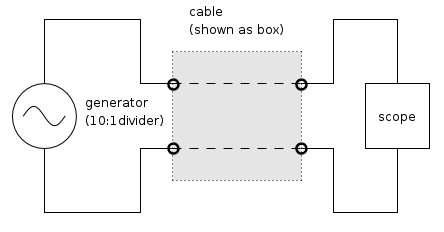
\includegraphics[scale = 0.65]{schaltung-leitung-01.png}
		\caption{\centering  Schaltung zur Untersuchung von hochfrequenten Signalen auf verschiedener Kabeln (erstellt mit GeoGebra)\\ (Box wird hier durch das jeweilige Kabel ersetzt)}
		\label{schaltung-leitungen}
	\end{figure}

	Wie zu sehen, wurde ein 10:1-Teiler an den Ausgang des Generators angeschlossen.
	Dieser verhindert die Beschädigung des Generators, sollten stehende Wellen oder andere Reflexionen bei der Messung auftreten, die in den Generator zurückgeführt werden könnten.
	Der Teiler verringert zwar die zu messende Spannung, wirkt sich aber nicht auf die zu beobachtenden Effekte aus. \\

	Für die Untersuchung von Impulsen auf Leitungen sollen die folgenden beiden Schaltungen in den Abbildungen \ref{schaltung_impuls_1} und \ref{schaltung_impuls_2} verwendet werden.
	Die Idee hierbei ist, die Laufzeit des Rechteckimpulses so zu verlängern, dass Reflexionen, welche am Ende des langen Koaxialkabels bzw. des Stichkabels auftreten, im Oszilloskop sichtbar werden.
	Aus diesem Grund soll für das Stichkabel ein vergleichsweise langes Koaxialkabel verwendet werden.

	\begin{figure}[H]
		\center
		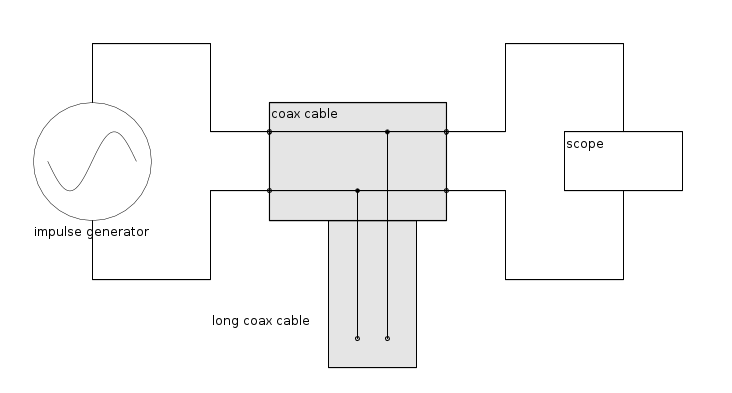
\includegraphics[scale = 0.8]{schaltung-impuls-01.png}
		\caption{\centering Erste Schaltung zur Untersuchung von Impulsen auf Leitungen (erstellt mit GeoGebra)}
		\label{schaltung_impuls_1}
	\end{figure}

	Um sich im Nachhinein auch das Ende des Stichkabels für verschiedene Fälle (angepasst und nicht angepasst) ansehen zu können, wurde dieses in der zweiten Schaltung ebenfalls an das Oszilloskop angeschlossen.
	Durch Veränderung des Eingangswiderstands von Channel 2 lassen sich hier verschiedene Anpassungen realisieren.

	\begin{figure}[H]
		\center
		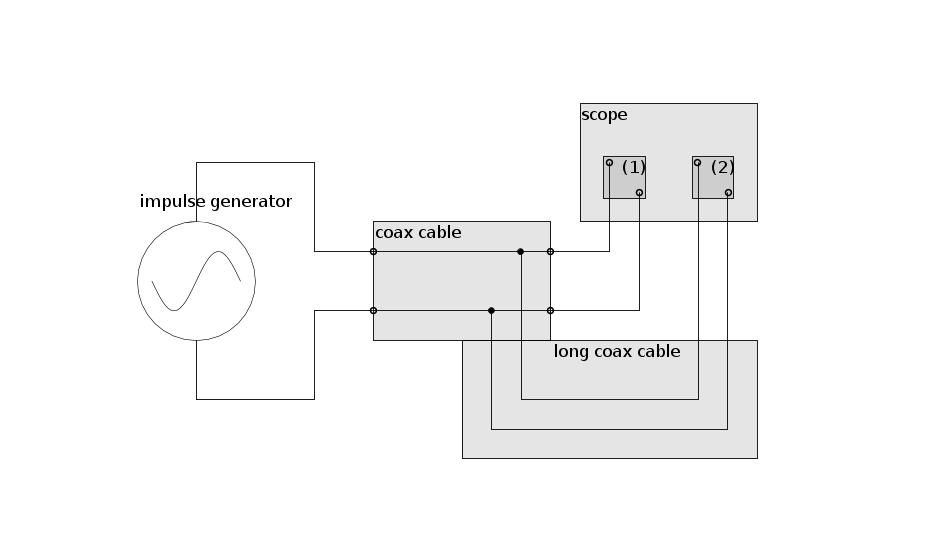
\includegraphics[scale = 0.8]{schaltung-impuls-02.png}
		\caption{\centering Zweite Schaltung zur Untersuchung von Impulsen auf Leitungen (erstellt mit GeoGebra)}
		\label{schaltung_impuls_2}
	\end{figure}

	Diese beiden Schaltungen lassen sich nun abändern, sodass der Wellenwiderstand des Stichkabels ermittelt werden kann.
	Dies wird erreicht, indem man am Ende des Stichkabels ein Potentiometer anschließt.
	Nach dem Anpassungsgesetz sollten gerade dann keine Reflexionen mehr beobachtbar sein, wenn der ohmsche Widerstand des Potentiometers dem Wellenwiderstand entspricht.
	Erreicht man also eine Einstellung, bei der keine Reflexionen auftreten, reicht es den ohmschen Widerstand auszumessen.\cite{unterlagen}

% subsection elektromagnetische_wellen_auf_leitungen (end)

\subsection{Modulation und Mischung} % (fold)
\label{sub:modulation_und_mischung}

	Für die Realisierung der in den Grundlagen besprochenen additiven Amplitudenmodulation wurde die Schaltung aus Abbildung \ref{schaltung_modulation_1} verwendet.
	Diese ermöglicht eine Analyse des Frequenzspektrums und des Zeitverlaufs.

	\begin{figure}[H]
		\center
		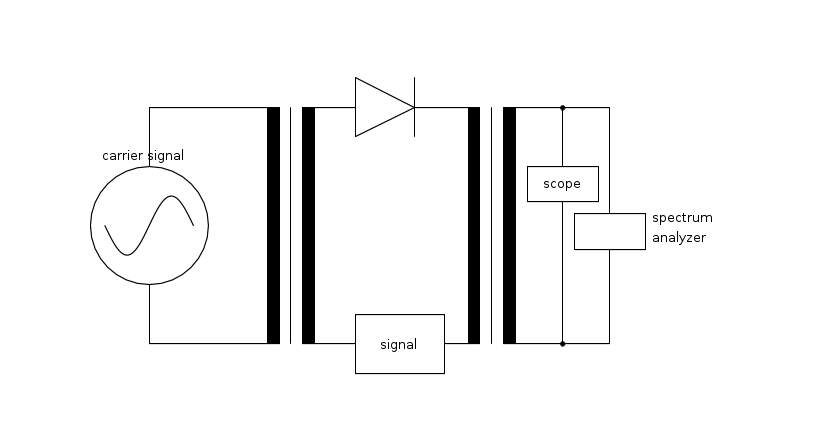
\includegraphics[scale = 1.0]{schaltung-modulation-01.png}
		\caption{\centering Schaltung für die Realisierung einer additiven Amplitudenmodulation \cite{unterlagen} (erstellt mit GeoGebra)}
		\label{schaltung_modulation_1}
	\end{figure}

	Eine nachfolgende Demodulationsschaltung wird in Abbildung \ref{schaltung_demodulation_1} gezeigt. 
	Das Signal wird wie in den Grundlagen beschrieben an einer Diode verzerrt und über einen Tiefpass geschickt.
	Das nachfolgende Spektrum enthält dann nur noch die tiefen Nutzfrequenzen. 

	\begin{figure}[H]
		\center
		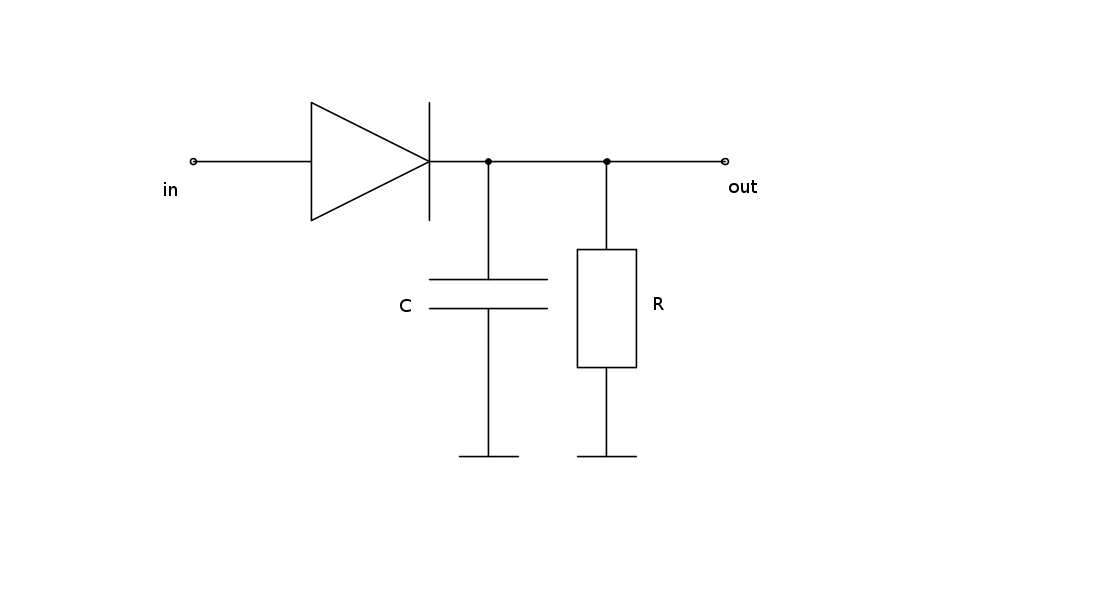
\includegraphics[scale = 0.5]{schaltung-demodulation-01.png}
		\caption{\centering Schaltung zur Realisierung einer Demodulation \cite{unterlagen} (erstellt mit GeoGebra)}
		\label{schaltung_demodulation_1}
	\end{figure}

% subsection modulation_und_mischung (end)

\subsection{Elektromagnetische Wellen im freien Raum} % (fold)
\label{sub:elektromagnetische_wellen_im_freien_raum}

	\subsubsection{Frequenzanpassung für eine Antenne} % (fold)
	\label{ssub:frequenzanpassung_f_r_eine_antenne}
	
		Aufgrund der in den Grundlagen betrachteten Theorie zu Antennen ist es klar, dass jede Antenne nur für bestimmte Frequenzen optimiert ist.
		Um diese Frequenzen zu bestimmen, soll ein Reflektometer verwendet werden.
		Folgende Schaltung in Abbildung \ref{schaltung_reflektometer_1} veranschaulicht dies.

		\begin{figure}[H]
			\center
			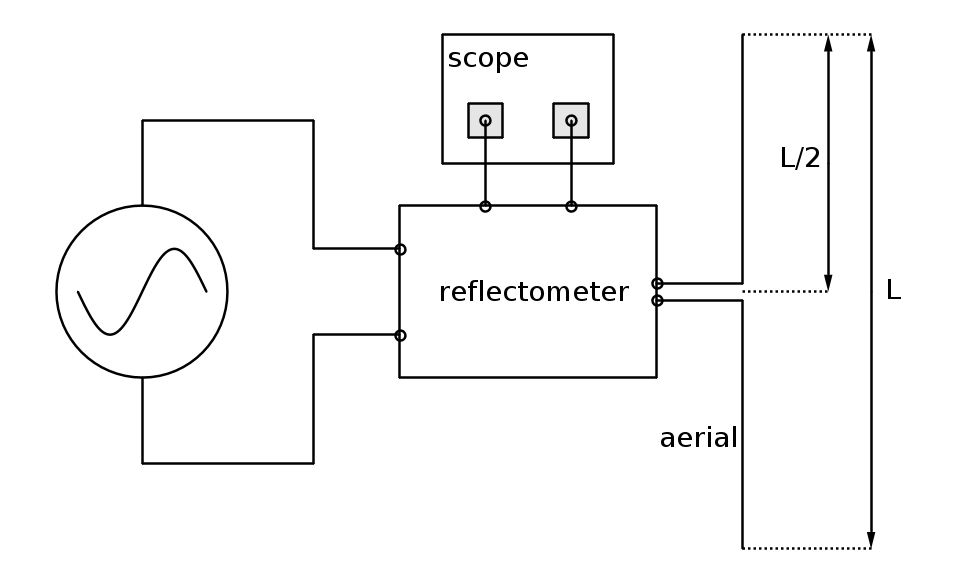
\includegraphics[scale = 0.35]{schaltung-reflektometer-01.png}
			\caption{\centering Schaltung zur Anpassung der Frequenz an eine Antenne mit der Länge $L$ unter Verwendung eines Reflektometers (erstellt mit GeoGebra)}
			\label{schaltung_reflektometer_1}
		\end{figure}

		Im Oszilloskop wird sowohl die rücklaufende als auch die hinlaufende Welle angezeigt.
		Während der Durchführung wurde nun versucht, das rücklaufende Signal so gering wie möglich zu wählen.
		Dies ermöglicht eine genaue Frequenzanpassung ohne eine theoretische Berechnung.\cite{unterlagen}

	% subsubsection frequenzanpassung_f_r_eine_antenne (end)

	\subsubsection{Senden und Empfangen von Signalen} % (fold)
	\label{ssub:senden_und_empfangen_von_signalen}
	
		Das Senden und Empfangen von Signalen soll einfach durch zwei Antennen realisiert werden.
		Hierbei wurde an die Erste ein Signal mit angepasster Frequenz angelegt.
		Durch ein Oszilloskop, welches an die zweite Antenne angeschlossen wurde, kann nun die Signalübertragung graphisch dargestellt werden.
		In Abbildung \ref{schaltung_antennen_1} sieht man die Details.

		\begin{figure}[H]
		 	\center
		 	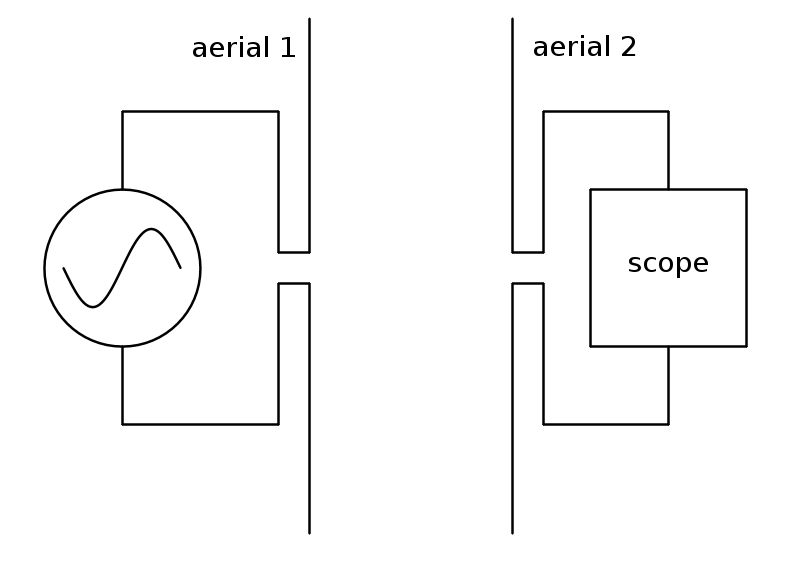
\includegraphics[scale = 0.4]{schaltung-antennen-01.png}
		 	\caption{\centering Grundsätzliche Schaltung für die Untersuchung des Sendens und Empfangens von Signalen über Antennen (erstellt mit GeoGebra)}
		 	\label{schaltung_antennen_1}
		\end{figure}

		In einem letzten qualitativen Versuchsteil, wurde mithilfe dieser grundsätzlichen Schaltung ein Audio-Signal übertragen.
		Dafür wurde dieses Signal auf eine angepasste Frequenz moduliert und dann nach Empfangen wieder demoduliert und abgespielt.
		Ersetzt man den Generator durch die Quelle des modulierten Audio-Signales und das Oszilloskop durch einen Demodulator in Verbindung mit einem Lautsprecher (oder einem Frequenzanalysator), so erhält man die für diesen Versuchsteil genutzte Schaltung.

		\cite{unterlagen}

	% subsubsection senden_und_empfangen_von_signalen (end)

% subsection elektromagnetische_wellen_im_freien_raum (end)